% Shared preamble for the English summaries in this repository.
\documentclass[11pt,a4paper]{article}
\usepackage[margin=2.2cm]{geometry}
\usepackage[T1]{fontenc}
\usepackage[utf8]{inputenc}
\usepackage{lmodern}
\usepackage{amsmath,amssymb}
\usepackage{graphicx}
\usepackage{booktabs}
\usepackage{enumitem}
\usepackage[hidelinks]{hyperref}
\setlist{itemsep=2pt,topsep=4pt}
\setlength{\parindent}{0pt}
\setlength{\parskip}{5pt}
\graphicspath{{figures/}}
\newcommand{\summaryheader}[3]{%
  \begin{center}
    {\Large\bfseries #2}\\[3pt]
    {\large #1}\\[3pt]
    {\small Arshia Goshtasbi \textbullet{} MSc Electrical Engineering (Control), Iran University of Science and Technology \textbullet{} #3}
  \end{center}
  \vspace{2pt}\hrule\vspace{8pt}
  \noindent\textit{English summary of my original Persian report, which is kept as a PDF in this folder.}\par}

\begin{document}
\summaryheader{Convex Optimization, Homework 1}{Optimization Basics, Chebyshev Approximation and Conic Fitting}{Spring 1404 (2025)}

\section*{Conceptual questions}
\begin{itemize}
  \item \textbf{The standard problem.} In $\min f_0(x)$ s.t.\ $f_i(x)\le 0$, the decision variable lives in $\mathbb{R}^n$, the domains of the $f_i$ are subsets of $\mathbb{R}^n$, and the functions are real-valued.
  \item \textbf{Chebyshev (minimax) approximation.} $\min_x \max_i |a_i^Tx-b_i|$ minimises the worst error instead of the sum of squares. With an auxiliary variable $t$ and the pairs of constraints $-t\le a_i^Tx-b_i\le t$ it becomes an LP. It shows up in data fitting, filter design and robust control. I also sketched a minimax model for crowding in a metro station.
  \item \textbf{Infimum versus minimum.} $1/x$ on $x>0$ has infimum $0$ but no minimum, and it has no maximum.
  \item \textbf{Facility location.} I formulated the best location of a petrol station among three points as a location (minimax or median) problem. Under an equal-distance criterion the answer is the incentre of the triangle, which is a convex combination of the three points.
  \item \textbf{Why convexity matters.} Every local optimum is global, interior-point methods solve convex problems in polynomial time, duality gives sensitivity information, and many practical problems (least squares, LP, SDP) are convex or can be made convex. I also defined global optima, local optima and sub-optimal solutions.
\end{itemize}

\section*{Fitting a conic to data (\texttt{Q2.m})}
The points in \texttt{data.mat} should lie on a conic $Ax^2+Bxy+Cy^2+Dx+Ey+F=0$. Each point gives one row $[x_i^2,\ x_iy_i,\ y_i^2,\ x_i,\ y_i,\ 1]$ of a matrix $M$. To avoid the trivial solution I fixed $F=1$. That leaves an ordinary least-squares problem $\min_\alpha\|M'\alpha+\mathbf{1}\|_2$ for $\alpha=(A,B,C,D,E)$, where $M'$ is the first five columns of $M$. Re-running the script gives
\[
A=-0.0404,\quad B=0.0011,\quad C=-0.1071,\quad D=0.0173,\quad E=0.0498,\quad F=1,
\]
an ellipse that passes through the data:
\begin{center}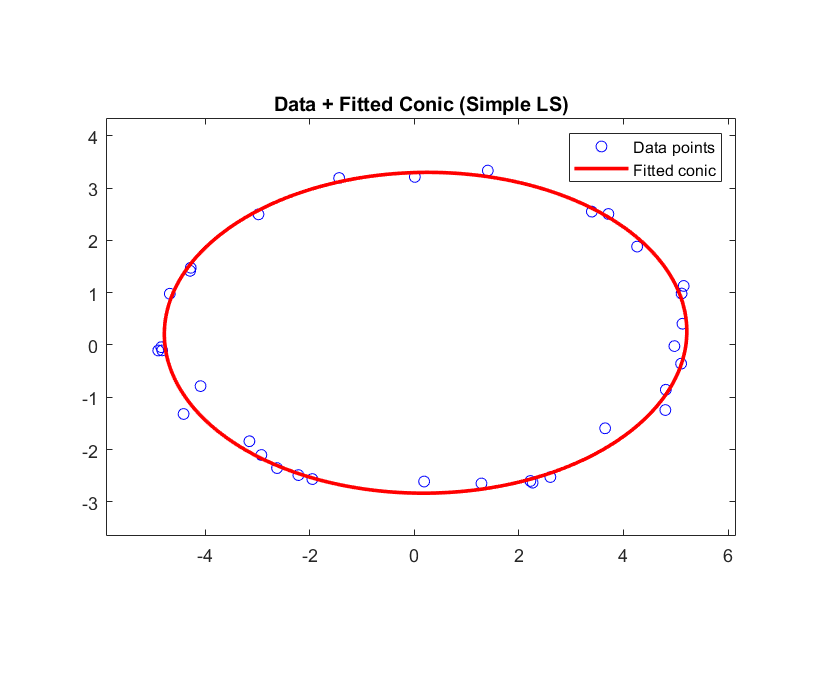
\includegraphics[width=0.55\linewidth]{Q2_1.png}\end{center}

\section*{Lamp illumination}
For the lamp problem I wrote three formulations:
\begin{itemize}
  \item making one point brighter than the average illumination;
  \item minimising total lamp power when any 5 of the 10 lamps together may use at most a given fraction of the power;
  \item using a single lamp to light every point.
\end{itemize}
\end{document}
